\begin{figure*}
    \centering
    \begin{subfigure}{0.46\textwidth}
        \centering
        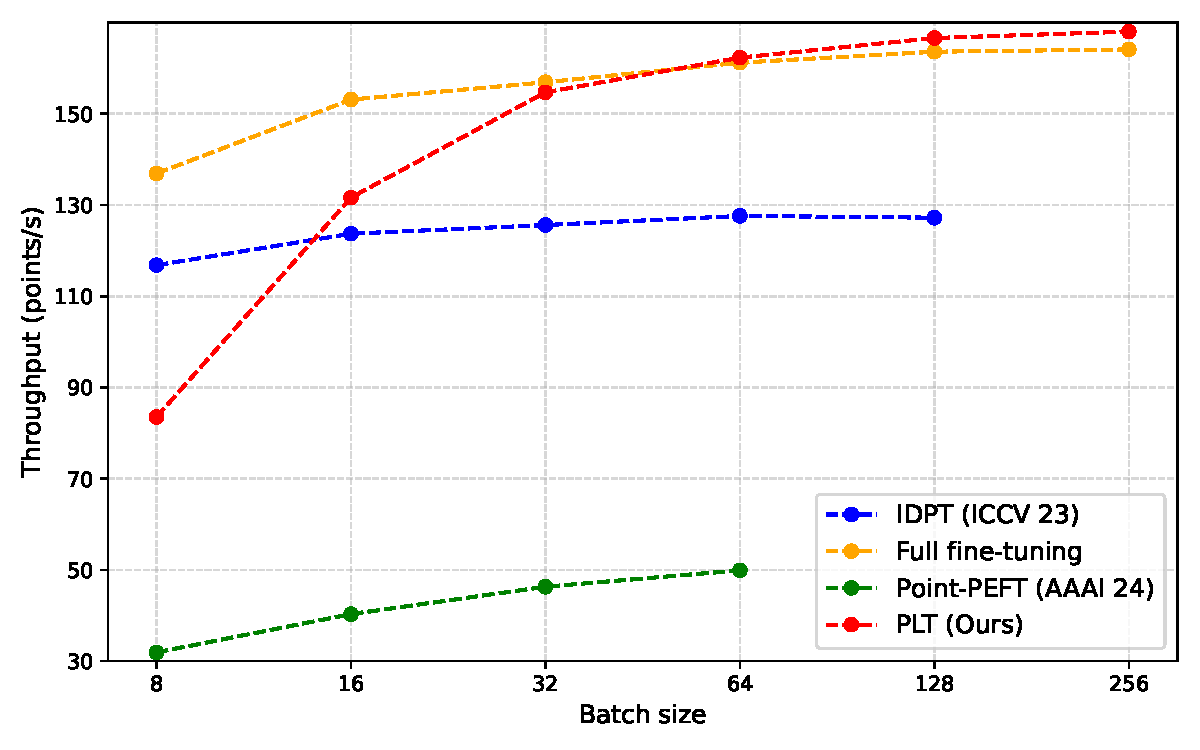
\includegraphics[width=\linewidth]{fig/supplement/performance/train_speed.pdf}
        \caption{Train Speed}
        \label{fig:per1}
    \end{subfigure}
    \hfill
    \begin{subfigure}{0.46\textwidth}
        \centering
        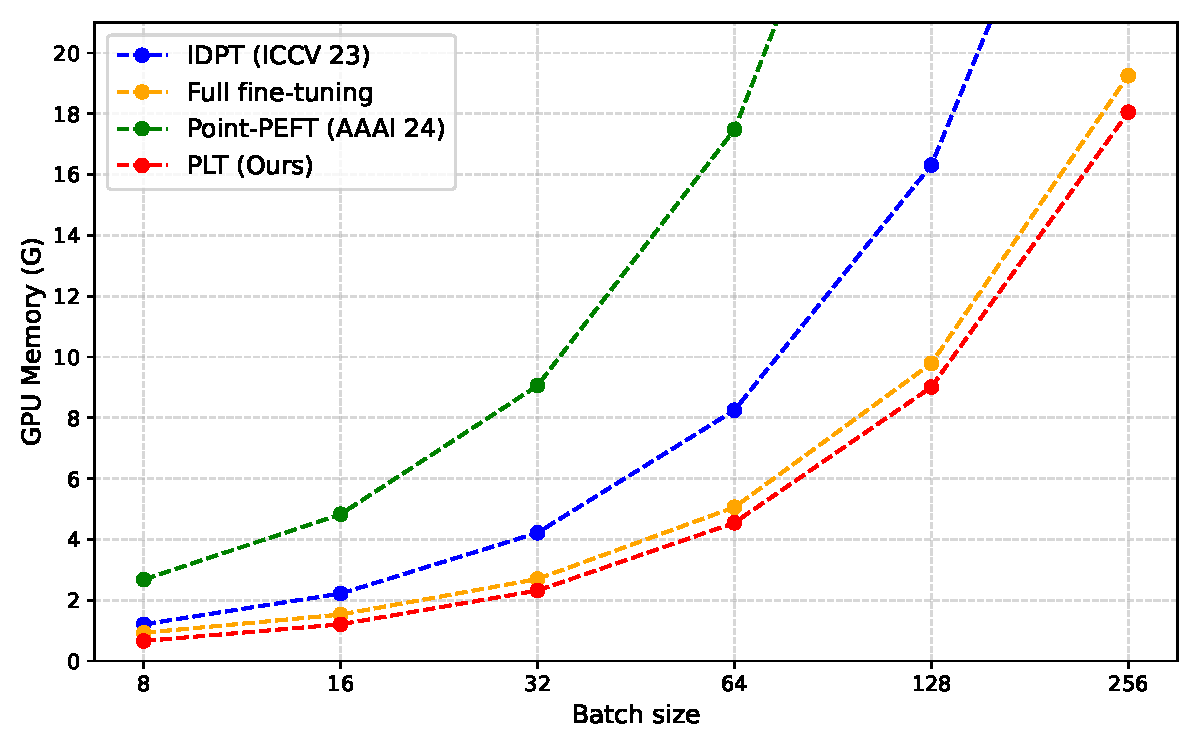
\includegraphics[width=\linewidth]{fig/supplement/performance/train_memory.pdf}
        \caption{Train Memory}
        \label{fig:per2}
    \end{subfigure}
    \hfill
    \begin{subfigure}{0.46\textwidth}
        \centering
        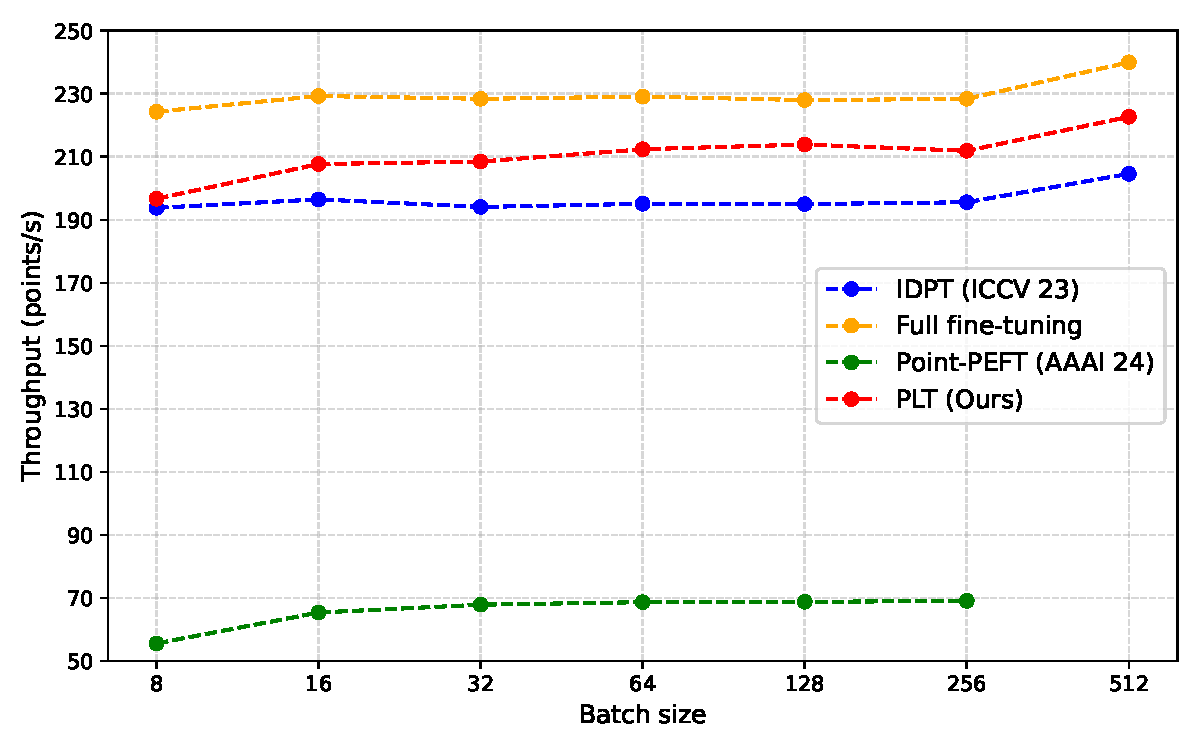
\includegraphics[width=\linewidth]{fig/supplement/performance/infer_speed.pdf}
        \caption{Infer Speed}
        \label{fig:per3}
    \end{subfigure}
    \hfill
    \begin{subfigure}{0.46\textwidth}
        \centering
        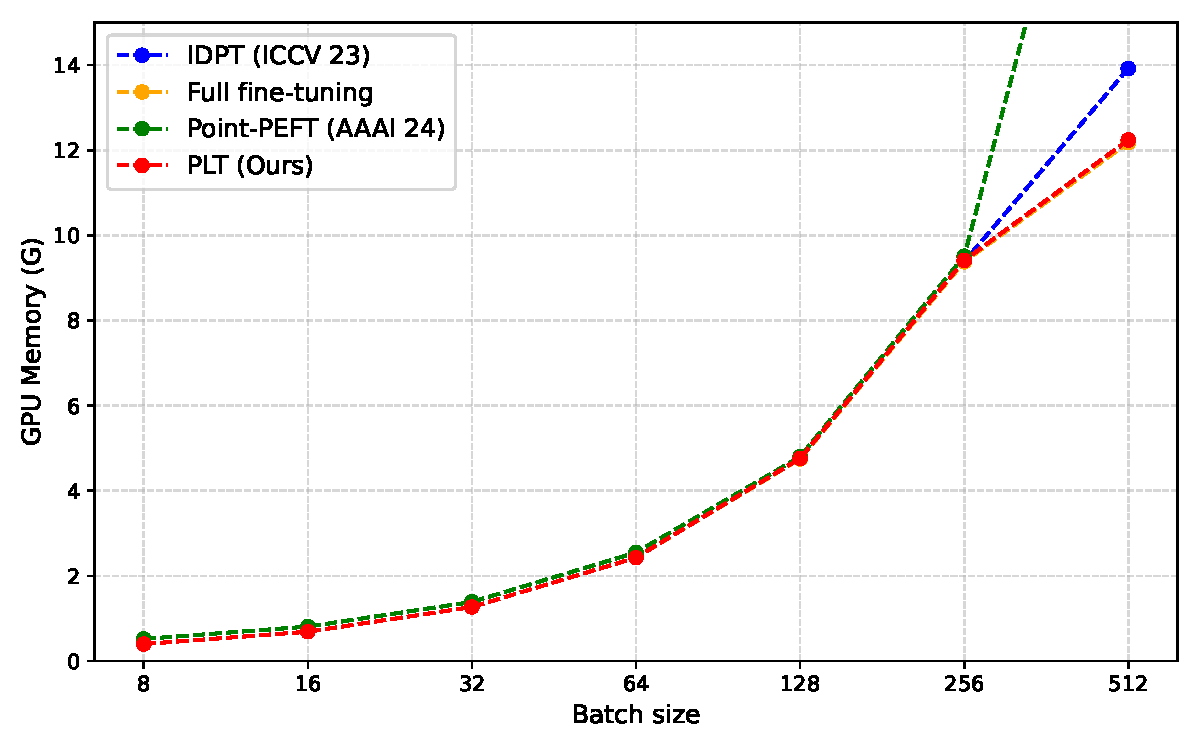
\includegraphics[width=\linewidth]{fig/supplement/performance/infer_memory.pdf}
        \caption{Infer Memory}
        \label{fig:per4}
    \end{subfigure}
    \hfill
    \caption{Comparison of performance between our PLT and previous methods. We conduct experiments on the hardest variant (i.e., PB\_T50\_RS) of ScanObjectNN~\cite{uy2019revisiting} with Point-MAE baseline~\cite{pang2022masked}. Throughput (points/s) is measured on single RTX 3090 GPU.}
    \label{fig:performance}
\end{figure*}